종현은 알고리즘 과제로 팰린드롬에 대해서 공부하고 있다. 팰린드롬(palindrome)이란 앞에서부터 읽으나 뒤에서부터 읽으나 같은 문자열을 말한다. 예를들어 'abba', 'level' 등은 팰린드롬이며 'abab', 'boj' 등은 팰린드롬이 아니다. 

\begin{center}
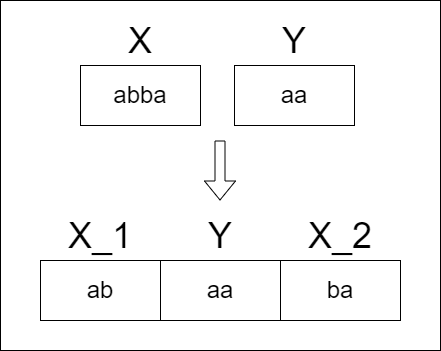
\includegraphics[bb=0 0 100 200]{draw.png}
\end{center}

종현은 팰린드롬을 보다가 새로운 현상을 발견하게 되었다. 먼저, \bf{길이가 짝수}인 문자열 $X$, $Y$를 고른다. 그리고 $X$를 같은 길이의 두 부분으로 나누어 문자열 $X_1$, $X_2$를 얻는다. 다음으로 종현은 $X_1$, $Y$와 $X_2$를 순서대로 이어 붙여 새로운 문자열 $Z$를 얻는다. 이렇게 얻은 $Z$가 팰린드롬이라면 종현은 $X$와 $Y$가 더블팰린드롬 현상을 일으킨다고 부르기로 했다. 길이가 짝수인 문자열 $N$개가 주어졌을 때 서로 다른 두 개의 문자열 $S{i}$, $S{j}$를 골라서 더블팰린드롬 현상을 만들 수 있는 쌍의 개수를 구하시오. 더블팰린드롬 현상에 관계없이 문자열 $S{i}$, $S{j}$가 다를 경우 다른 경우의 수로 둔다. 
